\section{A survey of the four fundamental projectors}
In the following pages we will look at three different kinds of mappings for a matrix $\Acc{m}{n}$: no frustration, frustration in one direction, frustration in both directions.

There are two different ways to view frustrated\index{frustration} mappings:
\begin{enumerate}
\item geometric deficiency\index{geometric deficiency} - mapping into a lower dimensional object;
\item algebraic deficiency\index{algebraic deficiency} - rank deficiency in row or column.
\end{enumerate}

In the examples that follow we will see ellipses mapped into other ellipses. These mappings are not frustrated. But once we map into a lower dimensional object, say from the unit sphere onto a line, the map is frustrated. This also means that we can't reverse the map. We can't make a finite linear map from a line with one parameter onto a sphere with three parameters.

These tables specify critical properties of the target matrix.

\textbf{Plots: }All plots start with the unit circle which is either
\begin{equation}
  \begin{array}{rcll}
     S(\theta) &=& \mat{c}{\cos \theta\\\sin \theta},\ \theta\in[0,2\pi) \qquad &n=2,\\
     S(\theta,\phi) &=& \mat{c}{\cos \theta\sin \phi\\\sin \theta \sin \phi\\\cos \phi},\ \theta\in[0,2\pi),\ \phi\in[0,\pi), \qquad &n=3.
  \end{array}
\end{equation}
Then look at the mapping action of the matrix. The result is either
\begin{equation}
  \A{}S(\theta) 
\end{equation}
when the target matrix has two columns or
\begin{equation}
  \A{}S(\theta,\phi) 
\end{equation}
when the target matrix has three columns.

The circles and ellipses have the color determined the the angular variable to provide an clearer idea of how the unit circle is distorted. So for the color red starts at $\theta=0$ and progresses through the spectrum until $\theta=2pi$ where the color is violet.\\

\textbf{Matrix images:} This block summarizes the plot above. For example, it may say that the plot represents a unit sphere being mapped to a line.\\

%%
\textbf{Vector space mappings:} These mappings are based on the dimensions of the spaces for the row and column vectors, $m$ and $n$. They disregard the issue of rank and and concerned purely with the mappings $\real{m}\mapsto\real{n}$ and  $\real{n}\mapsto\real{m}$. This map addresses the geometric deficiency of the mappings. For example are we going from a plane to a plane or a plane to a line. If the map is into a higher dimensional space we will have a frustrated map.\\

\textbf{Matrix ranks:} Are there rank deficiencies in the row or column space? If there is a rank deficiency we will see a frustrated map. 


\clearpage

%%
%% 2 x 2
%%
\begin{table}[htdp]
\begin{center}
\begin{tabular}{cc}
  $\A{}x=y$ & $\A{T}y=x$\\
$\mat{rr}{1&2\\-1&2}\mat{c}{x_{1}\\x_{2}} = \mat{c}{y_{1}\\y_{2}}$ &
$\mat{rr}{1&-1\\2&2}\mat{c}{x_{1}\\x_{2}} = \mat{c}{y_{1}\\y_{2}}$ \\
\ \\
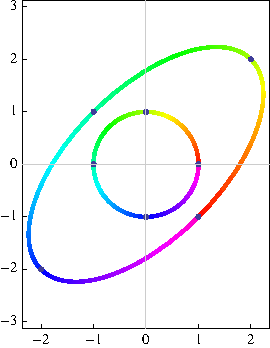
\includegraphics[ width = 2.15in ]{pdf/post_mortemII/2_2_2} &
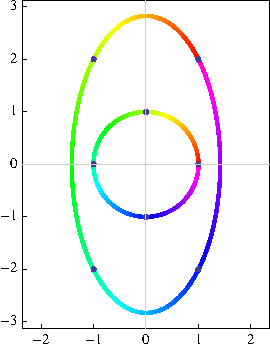
\includegraphics[ width = 2.15in ]{pdf/post_mortemII/2_2_2_t} \\
%%
\ \\
 $\Ap = \frac{1}{4}\mat{rr}{2&-1\\2&1}$ & $\paren{\A{T}}^{+} = \frac{1}{4}\mat{rr}{2&2\\-1&1}$ \\
\ \\
 $\projra = \itwo$ & $\projrat = \itwo$ \\
\ \\
 $\projrap = \mat{cc}{0&0\\0&0}$ & $\projratp = \mat{cc}{0&0\\0&0}$ \\
\ \\
 $\projna = \itwo$ & $\projnat = \itwo$ \\
\ \\
 $\projnap = \mat{cc}{0&0\\0&0}$ & $\projnatp = \mat{cc}{0&0\\0&0}$ \\
\end{tabular}
\end{center}
\label{tab:proj:a}
\caption{The four fundamental projectors for a full rank matrix and its transpose. There is no null space for either $\A{}$ or $\A{T}$.}
\end{table}%

\clearpage
%%
%% 2 x 3
%%
\begin{table}[htdp]
\begin{center}
\begin{tabular}{cc}
  $\A{}x=y$ & $\A{T}y=x$\\
$\mat{ccc}{0&3&0\\1&1&2}\mat{c}{x_{1}\\x_{2}\\x_{3}} = \mat{c}{y_{1}\\y_{2}}$ &
$\mat{cc}{0&1\\3&1\\0&2}\mat{c}{y_{1}\\y_{2}} = \mat{c}{x_{1}\\x_{2}\\x_{3}}$ \\
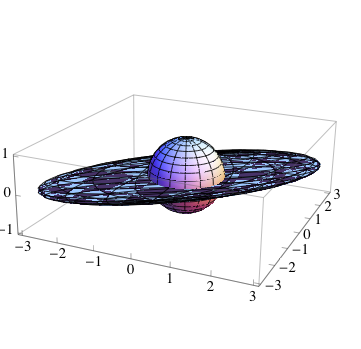
\includegraphics[ width = 2.5in ]{pdf/post_mortemII/3_2_2.png} &
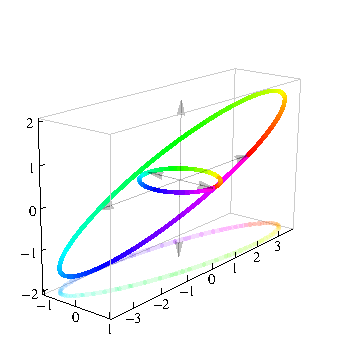
\includegraphics[ width = 2.5in ]{pdf/post_mortemII/3_2_2_t} \\
%%
 $\Ap = \frac{1}{15}\mat{rr}{-2&3\\5&0\\-4&2}$ & $\paren{\A{T}}^{+} = \frac{1}{5}\mat{rrr}{-2&5&-4\\3&0&2}$ \\
\ \\
 $\projra = \itwo$ & $\projrat = \frac{1}{5}\mat{ccc}{1&0&2\\0&1&0\\2&0&4}$ \\
\ \\
 $\projrap = \mat{cc}{0&0\\0&0}$ & $\projratp = \frac{1}{5}\mat{rrr}{4&0&-2\\0&\phantom{-}0&0\\-2&0&1}$ \\
\ \\
 $\projna = \frac{1}{5}\mat{ccc}{1&0&2\\0&1&0\\2&0&4}$ & $\projnat = \itwo$ \\
\ \\
 $\projnap = \frac{1}{5}\mat{rrr}{4&0&-2\\0&\phantom{-}0&0\\-2&0&1}$ & $\projnatp = \mat{cc}{0&0\\0&0}$ \\[15pt]
\end{tabular}
\end{center}
\label{tab:proj:b}
\caption{The four fundamental projectors for a matrix with full row rank. Because the target matrix has full row rank the range spans the domain space and  there is no perpendicular complement.}
\end{table}

\clearpage
%%
%% 3 x 2
%%
\begin{table}[htdp]
\begin{center}
\begin{tabular}{cc}
  $\A{}x=y$ & $\A{T}y=x$\\
$\Aexample \mat{c}{x_{1}\\x_{2}} = \mat{c}{y_{1}\\y_{2}\\y_{3}}$ &
$\Atexample\mat{c}{x_{1}\\x_{2}\\x_{3}} = \mat{c}{y_{1}\\y_{2}}$ \\
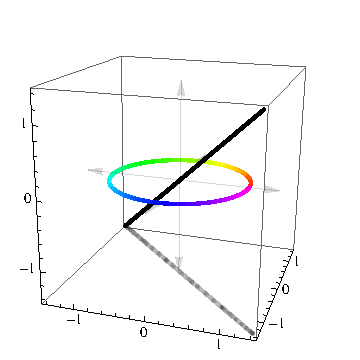
\includegraphics[ width = 2.5in ]{pdf/post_mortemII/3_2_1_a} &
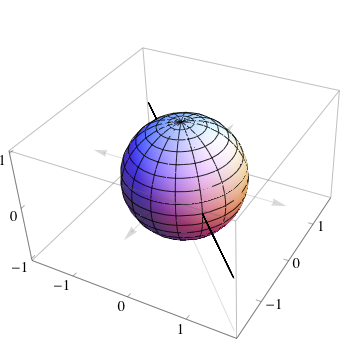
\includegraphics[ width = 2.5in ]{pdf/post_mortemII/3_2_1_t_a} \\
%%
 $\Ap = \Aplus$ & $\paren{\A{T}}^{+} = \frac{1}{6}\Aexample$ \\
\ \\
 $\projra = \frac{1}{3}\Aexample$ & $\projrat = \frac{1}{2}\mat{rr}{1&-1\\-1&1}$ \\
\ \\
 $\projrap = \frac{1}{3}\mat{rrr}{2&1&-1\\1&\phantom{-}2&1\\-1&1&2}$ & $\projratp = \frac{1}{2}\mat{rr}{1&1\\1&1}$ \\
\ \\
 $\projna = \frac{1}{2}\mat{rr}{1&-1\\-1&1}$ & $\projnat = \frac{1}{3}\Aexample$ \\
\ \\
 $\projnap = \frac{1}{2}\mat{rr}{1&1\\1&1}$ & $\projnatp = \frac{1}{3}\mat{rrr}{2&1&-1\\1&\phantom{-}2&1\\-1&1&2}$ \\[10pt]
\end{tabular}
\end{center}
\label{tab:proj:c}
\caption{The four fundamental projectors for a matrix with both row and column rank deficiences. Because the target matrix has full row rank the range spans the domain space and  there is no perpendicular complement.}
\end{table}
\clearpage
\endinput
